% The Merkle–Damgård iteration in SHA-2 [FIPS 180-4, §6.2.2, §6.4.2]: the padded message is
% split into blocks M^(1) ... M^(N); each block is compressed into the chaining value, starting
% from H^(0); the digest is the leftmost bits of H^(N).
% Original drawing for the Hash library.
\documentclass[tikz,border=6pt]{standalone}
\usepackage[T1]{fontenc}
\usepackage{lmodern}
% Shared style for the Hash diagrams.
% Palette: Okabe–Ito (colour-blind safe). Every diagram is drawn on an opaque white card so it
% stays legible on dark page themes.
\usetikzlibrary{arrows.meta,positioning,calc,fit,backgrounds}
\definecolor{hsblue}{HTML}{0072B2}
\definecolor{hsorange}{HTML}{E69F00}
\definecolor{hsgreen}{HTML}{009E73}
\definecolor{hsvermilion}{HTML}{D55E00}
\definecolor{hspurple}{HTML}{CC79A7}
\definecolor{hsink}{HTML}{1F2933}
\tikzset{
  >={Stealth[length=2.2mm]},
  every node/.style={font=\sffamily\small, text=hsink},
  wire/.style={draw=hsink, line width=0.6pt, ->},
  reg/.style={draw=hsink, line width=0.6pt, fill=hsblue!12, minimum width=9mm, minimum height=7mm},
  fn/.style={draw=hsink, line width=0.6pt, fill=hsorange!25, rounded corners=2pt, minimum width=10mm, minimum height=6mm},
  input/.style={draw=hsink, line width=0.6pt, fill=hsgreen!20, minimum width=9mm, minimum height=6mm},
  add/.style={circle, draw=hsink, line width=0.6pt, fill=white, inner sep=0pt, minimum size=5mm, font=\sffamily\bfseries},
  card/.style={fill=white, rounded corners=4pt},
}

\begin{document}
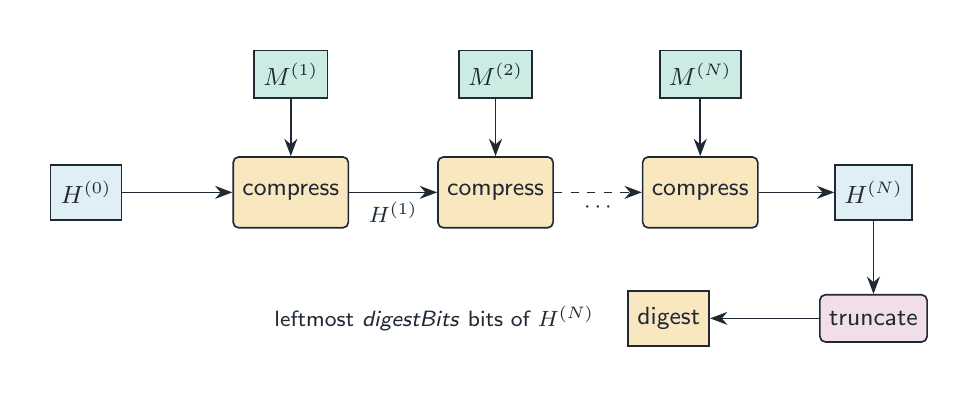
\begin{tikzpicture}
  \def\dx{2.6}
  \node[reg] (H0) at (0,0) {$H^{(0)}$};
  \foreach \i/\lbl in {1/1,2/2,3/N} {
    \node[fn, minimum width=14mm, minimum height=9mm] (C\i) at (\i*\dx, 0) {compress};
    \node[input] (M\i) at (\i*\dx, 1.5) {$M^{(\lbl)}$};
    \draw[wire] (M\i) -- (C\i);
  }
  \draw[wire] (H0) -- node[above, font=\sffamily\footnotesize] {} (C1);
  \draw[wire] (C1) -- node[below, font=\footnotesize] {$H^{(1)}$} (C2);
  \draw[wire, dashed] (C2) -- node[below, font=\footnotesize] {$\cdots$} (C3);
  \node[reg] (HN) at (4*\dx - 0.4, 0) {$H^{(N)}$};
  \draw[wire] (C3) -- (HN);
  \node[fn, fill=hspurple!25] (trunc) at (HN |- 0,-1.6) {truncate};
  \draw[wire] (HN) -- (trunc);
  \node[reg, fill=hsorange!25] (D) at ($(trunc)+(-\dx,0)$) {digest};
  \draw[wire] (trunc) -- (D);
  \node[font=\sffamily\footnotesize, anchor=east, text width=5.2cm, align=right] at ($(D.west)+(-0.3,0)$)
    {leftmost \textit{digestBits} bits of $H^{(N)}$};
  \begin{scope}[on background layer]
    \node[card, fit=(H0)(M3)(HN)(trunc), inner sep=8pt] {};
  \end{scope}
\end{tikzpicture}
\end{document}
